\section{Реализация принтера, основанного на шаблонах}

Основной целью данной работы была разработка прототипа принтера, который бы использовал для печати шаблоны.

\subsection{Описание общего подхода}

Работа принтера разбивается на два этапа: подготовка шаблонов и непосредственно печать синтаксического дерева.

На подготовительном этапе из файла с шаблонами языковых конструкций строится набор образцов. \textit{Образцом} назовем пару из текста шаблона и обобщенного синтаксического дерева шаблона. Дерево шаблона --- обобщенное, так как на месте некоторых узлов стоят специальные метки, которые хранят информацию об ограничениях на текстовое представление соответствующих узлов.

Во время основной фазы работы принтера дерево, которое необходимо непачатать, сравнивается с деревьями из образцов. В случае согласованности образца и дерева для печати используется текст образца, в который на места меток вставляются представления соответствующих поддеревьев.

% Благодаря шаблонам, необходимый результат получается просто и наглядно.

\subsection{Шаблон}

Внутри шаблона используется специальный язык разметки. Символы “\lstinline{@-}” на позиции поддерева синтаксической конструкции означают, что для применения данного шаблона поддерево должно быть напечатано в одну строку. Семантика символов “\lstinline{@* N @*}” совпадает с семантикой “\lstinline{@-}” с точностью до того, что напечатанное поддерево должно занимать строку длины не более N. Символы “\lstinline{@| @|}” означают, что соответствующее поддерево может быть напечатано и на нескольких строках. Для выделения отдельных шаблонов используются строки “\lstinline{t_start}”, “\lstinline{t_end}”.

Рассмотрим пример шаблонов для конструкции “\lstinline{write}” языка L (см. рис. \ref{fig:writeTmplt1} и \ref{fig:writeTmplt2}).
Эти шаблоны задают именно такое представление \lstinline{write}”, которого мы добивались в обзоре принтер-библиотек.

\begin{figure}[h!]
	\null\hfill
	\subfloat[]{
		\lstinputlisting{Podkopaev/codes/writeTmplt1.l}
		\label{fig:writeTmplt1}	
	}
	\hfill
	\subfloat[]{
		\lstinputlisting{Podkopaev/codes/writeTmplt2.l}
		\label{fig:writeTmplt2}
	}
	\hfill
	\null

	% \begin{subfigure}[h]{0.45\textwidth}
	% 	\lstinputlisting{Podkopaev/codes/writeTmplt1.l}
	% 	\caption{}
	% 	\label{fig:writeTmplt1}
	% \end{subfigure}
	% \begin{subfigure}[h]{0.45\textwidth}
	% 	\lstinputlisting{Podkopaev/codes/writeTmplt2.l}
	% 	\caption{}
	% 	\label{fig:writeTmplt2}
	% \end{subfigure}
	\caption{Шаблоны для конструкции “\lstinline{write}”}
\end{figure}

Рассмотрим шаблоны для конструкции “\lstinline{if-then-else}” (см. рис. \ref{fig:flatGoodIfTmplt} и \ref{fig:multBadIfTmplt}).
С помощью них можно напечатать дерево, изображенное на рисунке~\ref{fig:nestedIf} (см. рис. \ref{fig:nestedIfCode}).

\begin{figure}[h!]
	\subfloat[Однострочный вариант]{
		\lstinputlisting{Podkopaev/codes/flatGoodIfTmplt.l}
		\label{fig:flatGoodIfTmplt}
	}
	\hfill
	\subfloat[Многострочный вариант]{
		\lstinputlisting{Podkopaev/codes/multBadIfTmplt.l}
		\label{fig:multBadIfTmplt}
	}
	
	% \begin{subfigure}[h]{0.45\textwidth}
	% 	\lstinputlisting{Podkopaev/codes/flatGoodIfTmplt.l}
	% 	\caption{Однострочный вариант}
	% 	\label{fig:flatGoodIfTmplt}
	% \end{subfigure}
	
	% \begin{subfigure}[h]{0.45\textwidth}
	% 	\lstinputlisting{Podkopaev/codes/multBadIfTmplt.l}
	% 	\caption{Многострочный вариант}
	% 	\label{fig:multBadIfTmplt}
	% \end{subfigure}
	\caption{Шаблоны для конструкции “\lstinline{if-then-else}”}
	\label{fig:ifTmplt}
\end{figure}

\begin{figure}[h!]
	\centering
	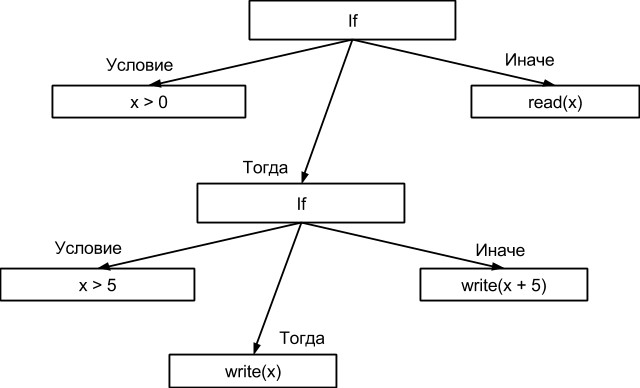
\includegraphics[width=0.6\textwidth]{nestedIf}
	\caption{Пример дерева “\lstinline{if-then-else}”}
	\label{fig:nestedIf}
\end{figure}

\begin{figure}[h!]
	\centering
	\lstinputlisting{Podkopaev/codes/nestedIf.l}
	\caption{Представление с помощью шаблонов с рис. \ref{fig:ifTmplt}}
	\label{fig:nestedIfCode}
\end{figure}

Одним из неочевидных свойств шаблонов является то, что с их помощью можно выражать не только базовые конструкции языка.
Например, можно завести отдельный шаблон для случая, когда обе ветки конструкции “\lstinline{if-then-else}” представляют собой операторы “\lstinline{write}” (см. рис. \ref{fig:writeNestedInIf}). Если добавить такой шаблон, то пример дерева с рисунка~\ref{fig:nestedIf} получит новое представление (см. рис. \ref{fig:nestedIfNew}).

\begin{figure}[h!]
	\lstinputlisting{Podkopaev/codes/writeNestedInIf.t}
	\caption{Пример задания шаблона для сложной конструкции}
	\label{fig:writeNestedInIf}
\end{figure}

\begin{figure}[h!]
	\lstinputlisting{Podkopaev/codes/nestedIfNew.l}
	\caption{Представление дерева с рис. \ref{fig:nestedIf} с использованием шаблона с рис. \ref{fig:writeNestedInIf}}
	\label{fig:nestedIfNew}
\end{figure}

\subsection{Построение образцов}

Для работы принтера неообходимо иметь возможность сравнивать синтаксическое представление шаблонов с деревом, которое печатается. Поэтому необходим синтаксический анализатор, который может разбирать шаблонные конструкции в рамках целевого языка. Удобным способом разработать данный анализатор является использование расширяемого синтаксического анализатора целевого языка. В результате работы расширенного анализатора получается набор образцов. В узлах синтаксического дерева, соответствующих меткам шаблонов, хранится информация о положении метки внутри текста образца, чтобы на этапе печати документа знать, куда вставлять представления поддеревьев.

\subsection{Печать дерева с использованием набора образцов}

На этапе, когда уже имеются необходимые образцы, происходит их сопоставление с синтаксическим деревом, переданным на печать.
Псевдокод алгоритма приведен ниже (см. рис. \ref{fig:comparePseudoCode}).

\begin{figure}
        \small
	\begin{algorithmic}
		\State{H --- ассоциативный массив, связывает деревья с их текстовым представлением}
		\State{M --- набор образцов для языковых конструкций}
		\State{По дереву строит его текстовое представление}
		\Function{print}{$tree$}
			\If{$tree \in H$}{ }\Return{$H[tree]$}
			\Else { Вызов print для поддеревьев $tree$}
			      {    }\State\Return{\Call{templateIter}{$tree$}}
			\EndIf
		\EndFunction
		\State{Перебирает все образцы и пытается их применить к дереву}
		\Function{templateIter}{$tree$}
			\ForAll{$(templateTree, text) \in M$}
				\State{В случае исключения, переходит к новому элементу $M$}
				\State{$list$ := \Call{templateCompare}{$tree, templateTree$}}
				\State{$H[tree]$ := построенное представление для $tree$ по $list$ и $text$}
				\State\Return{$H[tree]$}
			\EndFor
		\EndFunction
		\State{Возвращает список координат метки в тексте шаблона и соответствующее текстовое представление поддерева}
		\Function{templateCompare}{$tree, templateTree$}
			\If{$tree$ и $templateTree$ одного типа}
				\State{Вызвать $templateCompare$ для соответствующих поддеревьев}
				\State\Return{соединенный список результатов вызова для поддеревьев}
			\EndIf
			\If{$templateTree$ является меткой}
				\If{$H[tree]$ соответствует ограничениям метки}
					\State\Return{$[($координаты метки$, H[tree])]$}
				\Else{ создать исключение}
				\EndIf
			\EndIf
			\State{Создать исключение, т.к. переданные деревья разной структуры}
		\EndFunction		
	\end{algorithmic}
	\caption{Псевдокод сопоставления дерева с набором образцов}
	\label{fig:comparePseudoCode}
\end{figure}

Из псевдокода видно, что в случае, если для какого-нибудь поддерева не найдется соответствующий образец, то дерево невозможно будет напечатать. То есть множество образцов должно быть достаточным. Это естественное ограничение.

% Попробуем оценить время работы алгоритма. Пусть $|M|$ --- количество образцов, $height(T)$ --- высота дерева, а $K$ --- максимальное число поддеревьев у узла синтаксического дерева целевого языка. Тогда время работы алгоритма можно оценить как $O((|M| \times K)^{height(T)} )$.

Попробуем оценить время работы алгоритма. Для каждого узла дерева, переданного принтеру, вычисляется следующее:
\begin{enumerate}
	\item текстовое представление для детей;
	\item сравнение с имеющимися образцами;
	\item текстовое представление узла по выбранному образцу и представлениям детей.
\end{enumerate}

Текстовое представление вычисляется для каждого узла один раз. Сравнение с образцами занимает $O(B \times |M|)$ времени, где $B$ --- максимальное число узлов в дереве образца, а $|M|$ --- количество образцов. Построение текстового представления по выбранному образцу занимает $O(A)$, где $A$ --- максимальное количество меток в шаблоне, но так как очевидно, что $A \leq B$, то оценку можно заменить на $O(B)$. Таким образом, оценка на работу алгоритма для дерева с $T$ узлами равна $O(T \times B \times |M|)$.

Для сравнения, если реализовать аналогичный принтер с помощью библиотеки Азеро и Свиерстры, то это приведет к экспоненциальному от размера дерева расчету текстового представления. В случае библиотек Хьюза и Вадлера похожий принтер будет иметь квадратичную сложность.

\subsection{Реализованный принтер}

Описанный подход был реализован на примере принтера языка L, написанного на языке OCaml\footnote{http://ocaml.org}. Для написания синтаксического анализатора была использована библиотека Ostap\footnote{http://oops.math.spbu.ru/projects/ostap}.

В качестве примера работы принтера с разными шаблонами рассмотрим уже упоминавшуюся программу быстрого возведения в степень (см. рис. \ref{fig:lEx}).
С помощью шаблонов, приведенных в приложении~\ref{app:1}, принтер печатает программу в виде, изображенном на рисунке \ref{fig:firstTemplatePow}.

\begin{figure}[h!]
	\lstinputlisting{Podkopaev/codes/firstTemplatePow.l}
	\caption{Программа быстрого возведения в степень на языке L, напечатанная с помощью шаблонов из приложения~\ref{app:1}}
	\label{fig:firstTemplatePow}
\end{figure}

Шаблоны, приведенные в приложении~\ref{app:2}, представляют программу несколько иным образом (см. рис. \ref{fig:secondTemplatePow}).

\begin{figure}[h!]
	\lstinputlisting{Podkopaev/codes/secondTemplatePow.l}
	\caption{Программа быстрого возведения в степень на языке L, напечатанная с помощью шаблонов из приложения~\ref{app:2}}
	\label{fig:secondTemplatePow}
\end{figure}

Из приведенных примеров виден один из недостатков реализации. Если присмотреться к конструкции \lstinline{if-then-else}, то можно заметить, что \lstinline{then} и \lstinline{else} находятся на разных уровнях. Естественно, это нежелательный результат. Пока эта проблема не решена, в дальнейшем планируется разобраться с этой проблемой путем расширения языка шаблонов.
